%% res.tex
%% $Id: eval.tex 5 2005-10-10 20:55:48Z bless $

%%%%%%%%%%%%%
\chapter{Evaluation}
\label{ch:evaluation}
%%%%%%%%%%%%%

\section{Deskriptive Statistik}

\section{Beschreibung der Ergebnisse}

\subsection{Konstruktionsprinzip versus Konfigurationsprinzip}

\subsubsection{Konstruktionsprinzip}
\begin{figure}[h]
\centering
\includegraphics[width=1\textwidth]{pictures/konstruktion}
\caption{Architektur des \emph{konstruktion}}
\label{therapyBuilder}
\end{figure}

\subsubsection{Konfigurationsprinzip}

\begin{figure}[h]
\centering
\includegraphics[width=1\textwidth]{pictures/konfiguration}
\caption{Architektur des \emph{konfiguration}}
\label{therapyBuilder}
\end{figure}


\subsubsection{Gegenüberstellung}


\subsection{Sprünge versus Sichtbarkeitsregeln}

\subsubsection{Sprünge}
\begin{figure}[h]
\centering
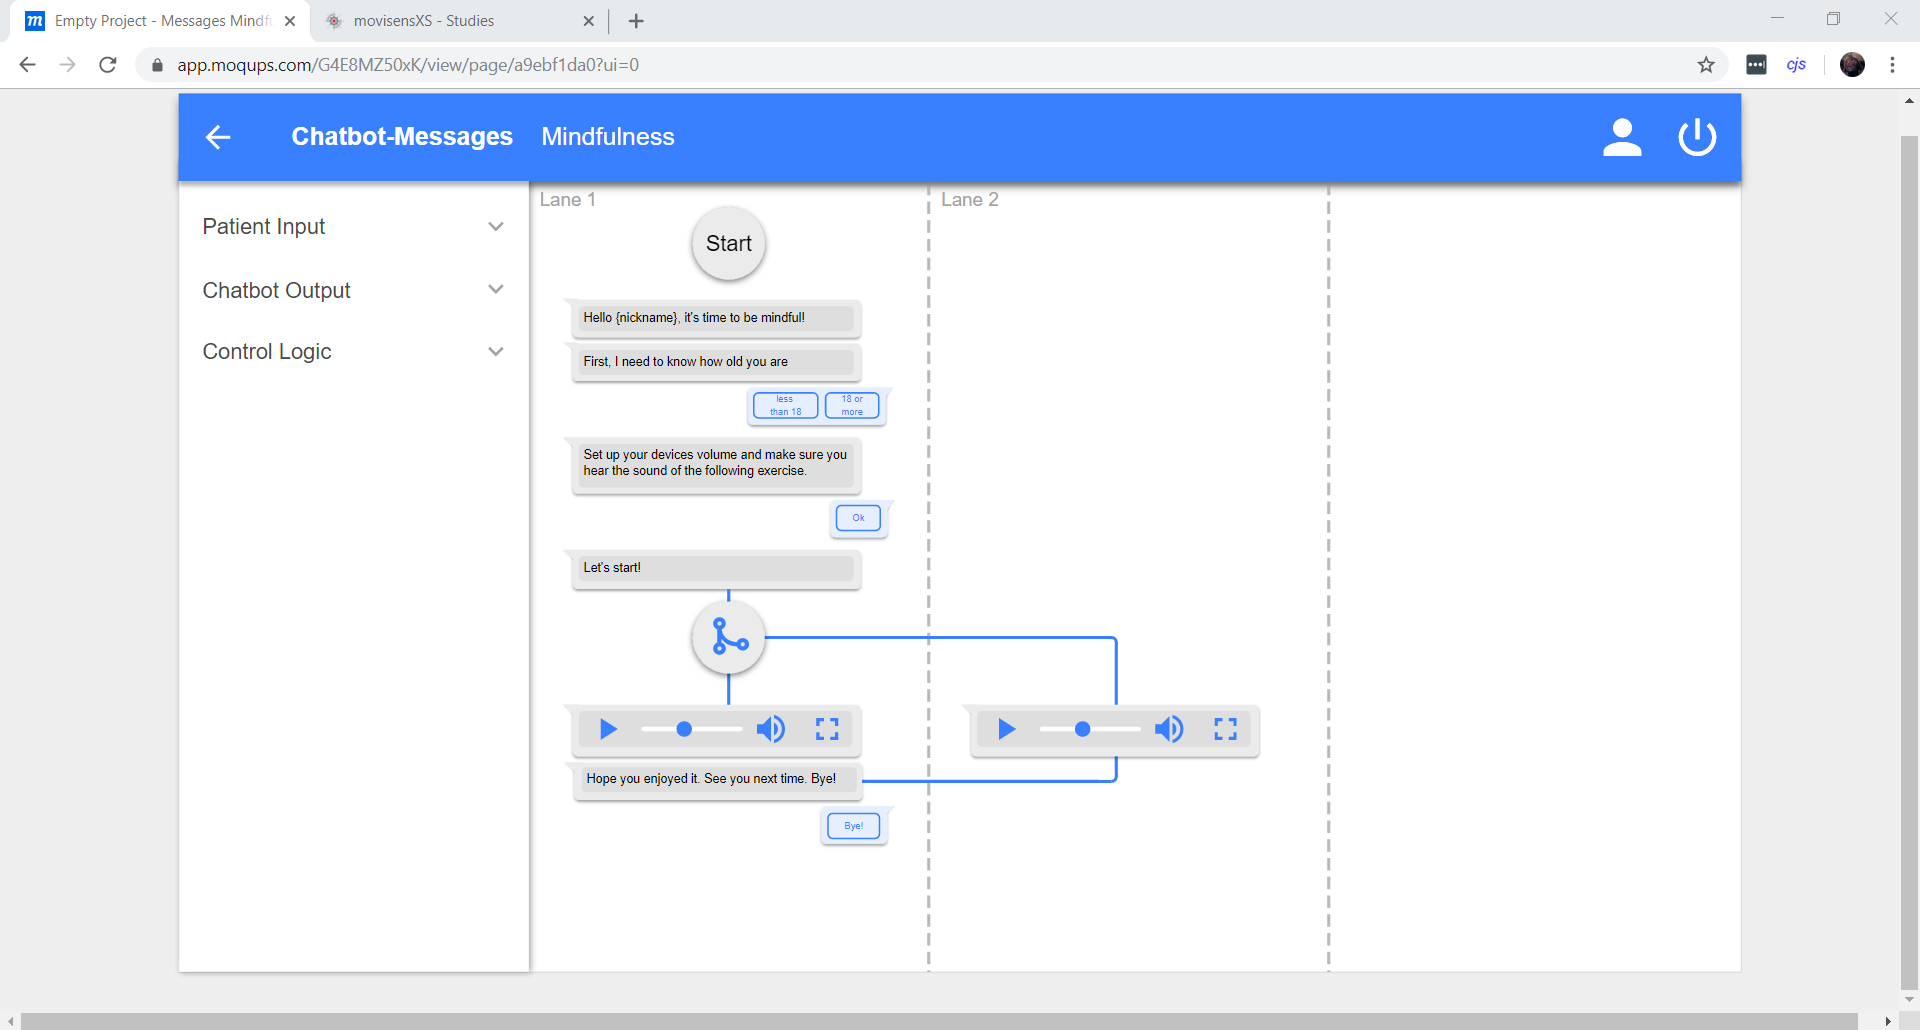
\includegraphics[width=1\textwidth]{pictures/spruenge}
\caption{Architektur des \emph{spruenge}}
\label{therapyBuilder}
\end{figure}


\subsubsection{Sichtbarkeitsregeln}

\begin{figure}[h]
\centering
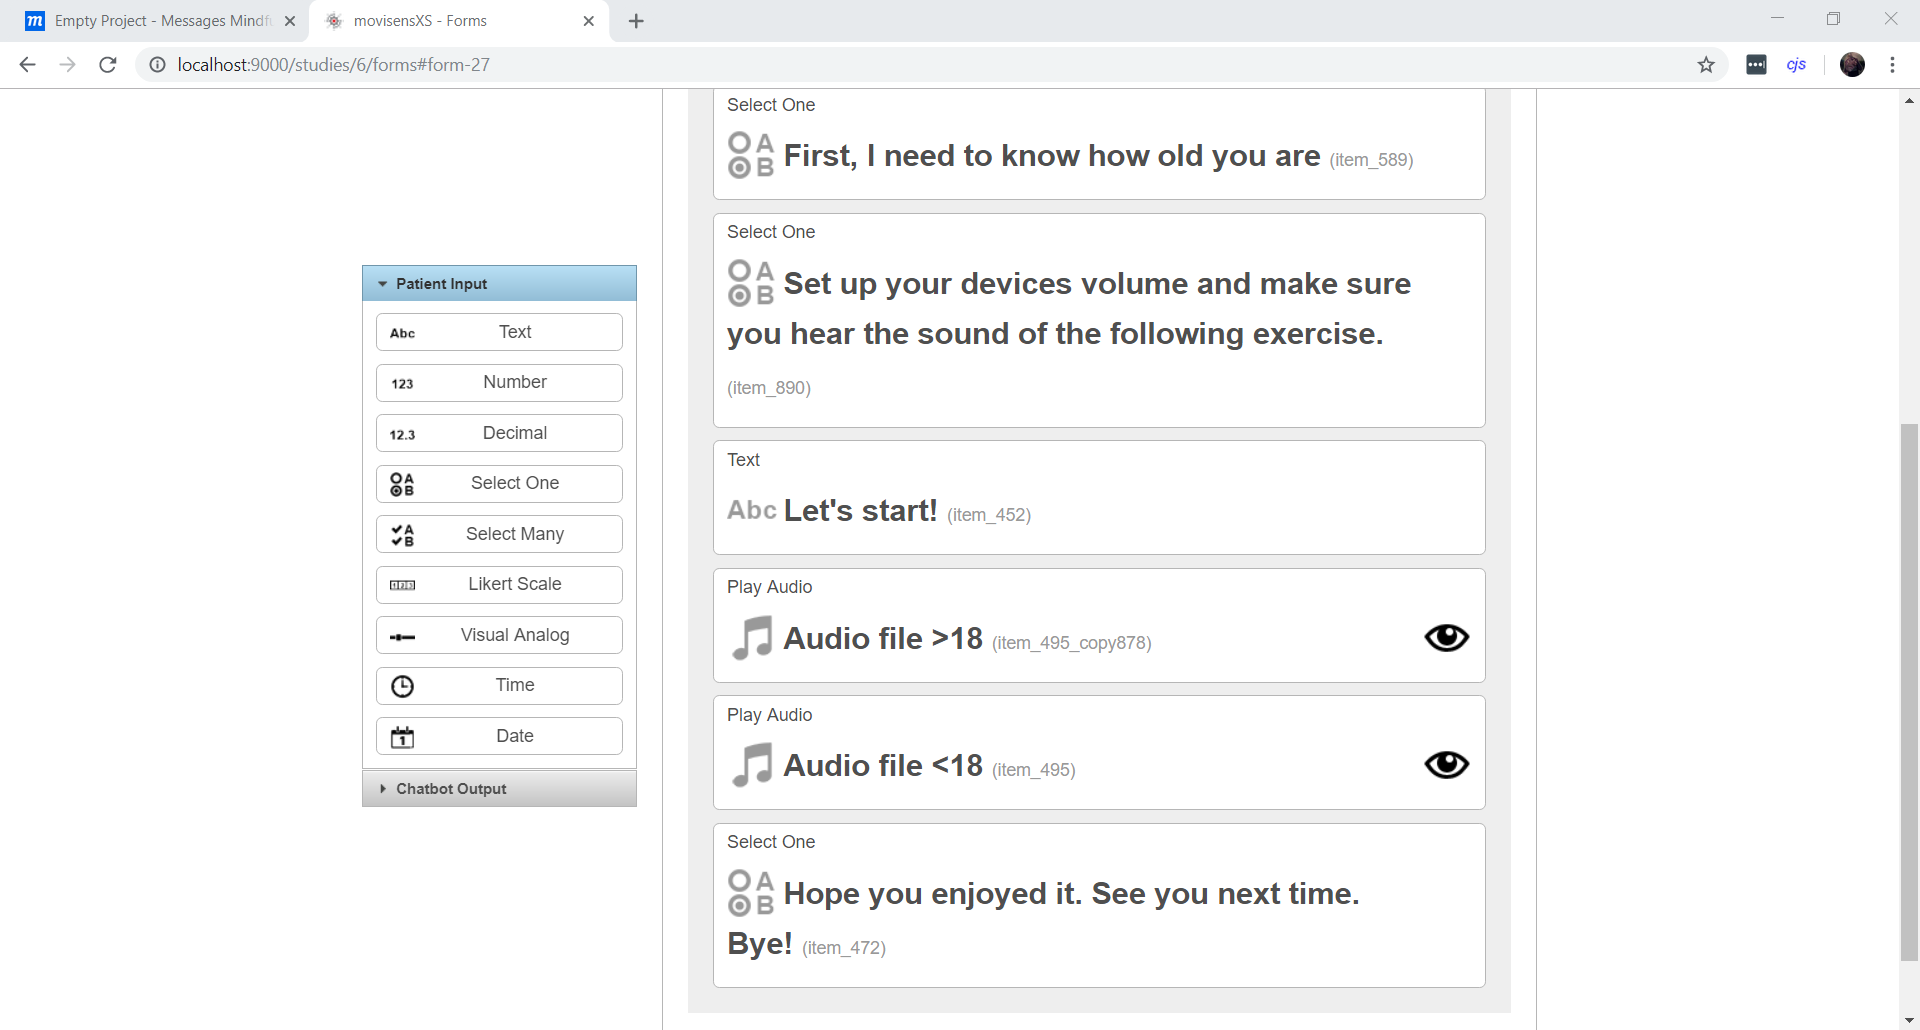
\includegraphics[width=1\textwidth]{pictures/sichtbarkeit}
\caption{Architektur des \emph{sichtbarkeit}}
\label{therapyBuilder}
\end{figure}


\subsubsection{Gegenüberstellung}

\begin{figure}[h]
\centering
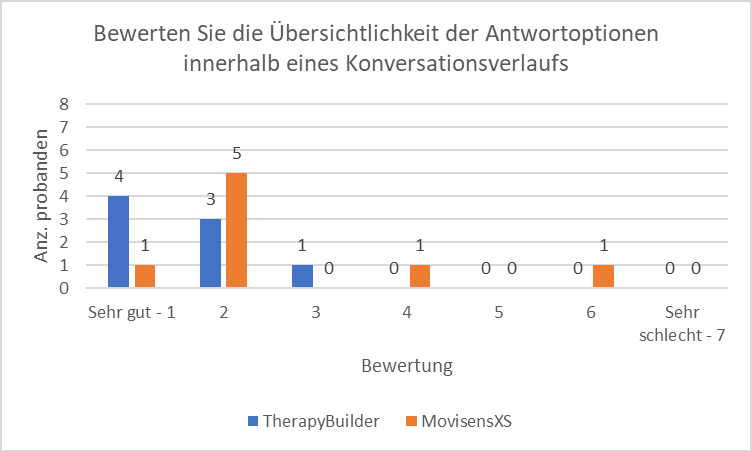
\includegraphics[width=1\textwidth]{pictures/diagramme/antwortoptkonv}
\caption{Architektur des \emph{sichtbarkeit}}
\label{therapyBuilder}
\end{figure}

\begin{figure}[h]
\centering
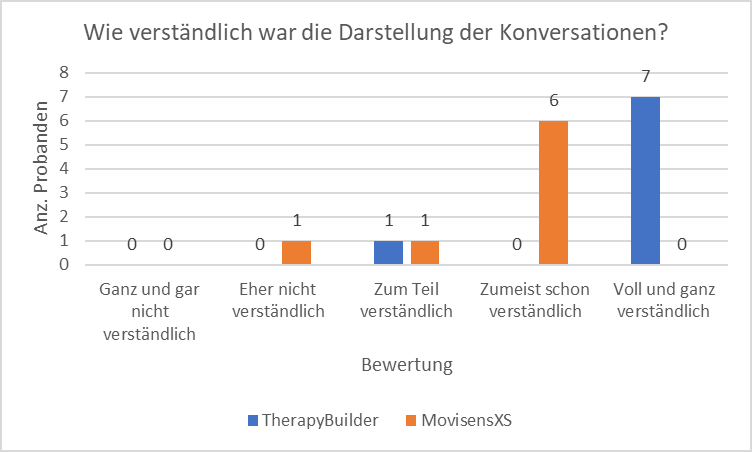
\includegraphics[width=1\textwidth]{pictures/diagramme/konversationdarstellung}
\caption{Architektur des \emph{konfiguration}}
\label{therapyBuilder}
\end{figure}

\begin{figure}[h]
\centering
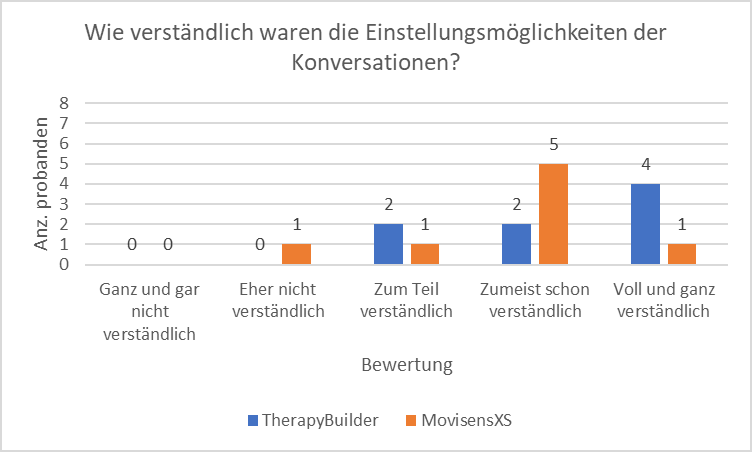
\includegraphics[width=1\textwidth]{pictures/diagramme/konversationeinstellung}
\caption{Architektur des \emph{konfiguration}}
\label{therapyBuilder}
\end{figure}

\begin{figure}[h]
\centering
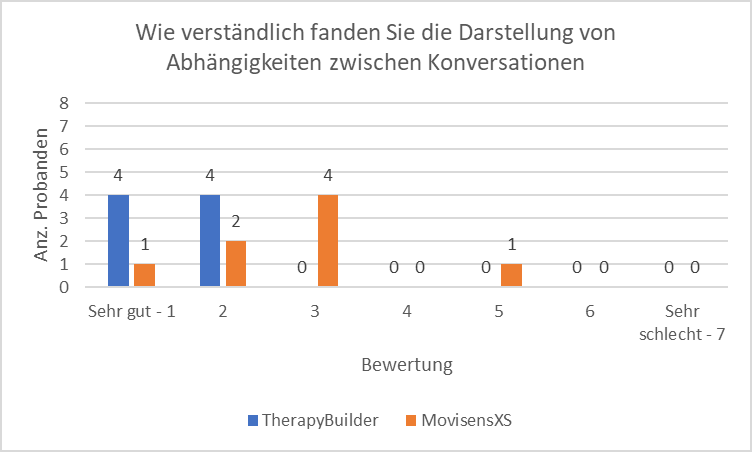
\includegraphics[width=1\textwidth]{pictures/diagramme/konversationenabhaeng}
\caption{Architektur des \emph{konfiguration}}
\label{therapyBuilder}
\end{figure}

\begin{figure}[h]
\centering
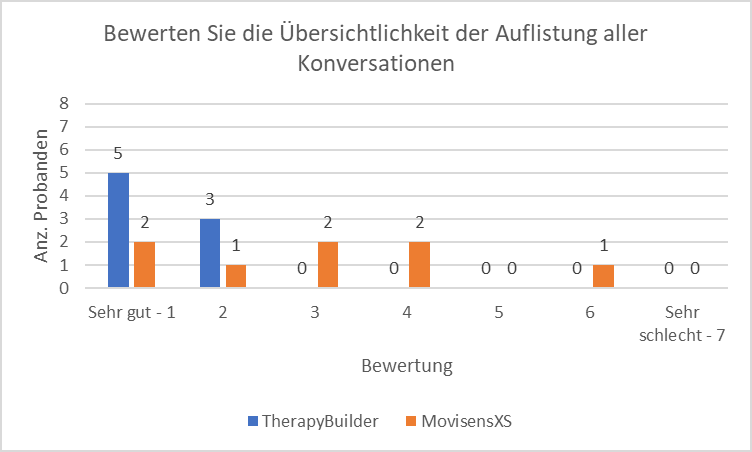
\includegraphics[width=1\textwidth]{pictures/diagramme/konversationenuebersicht}
\caption{Architektur des \emph{konfiguration}}
\label{therapyBuilder}
\end{figure}

\begin{figure}[h]
\centering
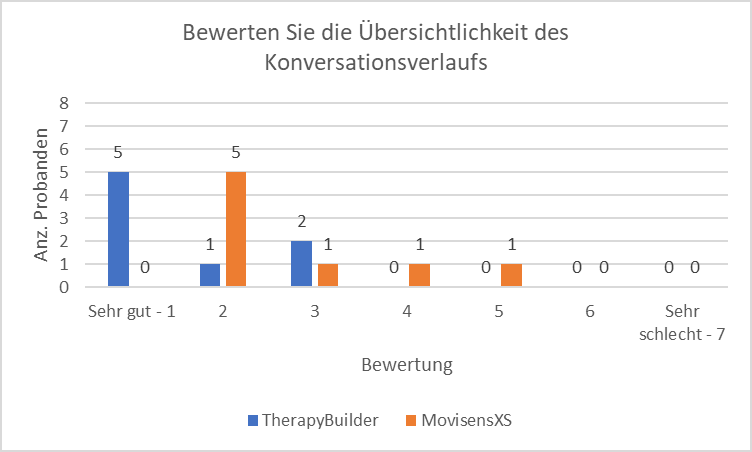
\includegraphics[width=1\textwidth]{pictures/diagramme/konversationverlfueber}
\caption{Architektur des \emph{konfiguration}}
\label{therapyBuilder}
\end{figure}

\begin{figure}[h]
\centering
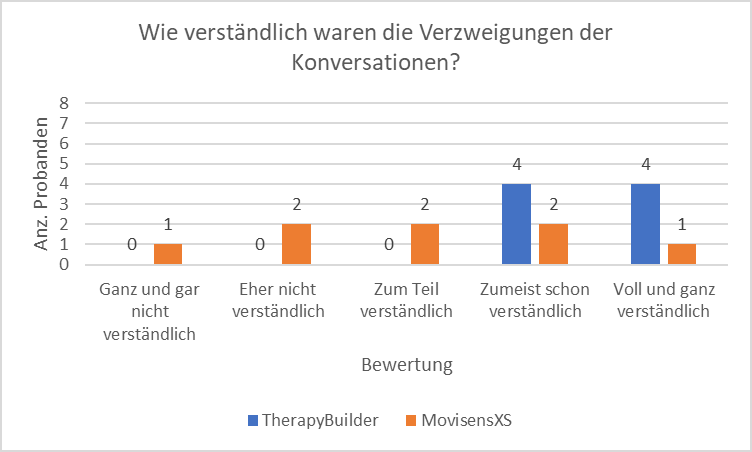
\includegraphics[width=1\textwidth]{pictures/diagramme/konversationverzweigung}
\caption{Architektur des \emph{konfiguration}}
\label{therapyBuilder}
\end{figure}

\begin{figure}[h]
\centering
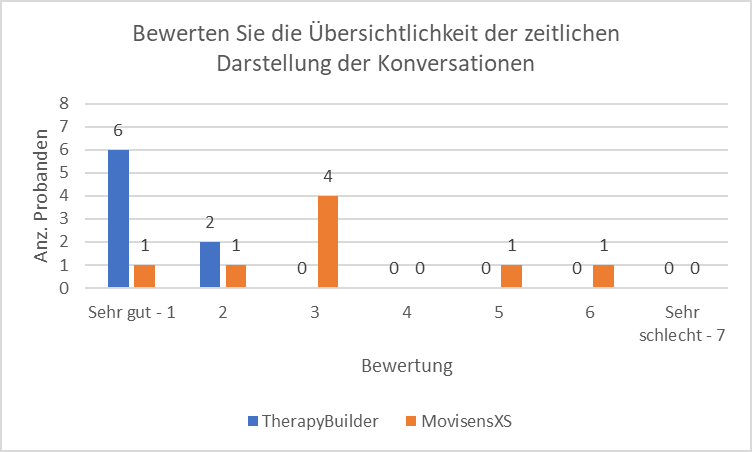
\includegraphics[width=1\textwidth]{pictures/diagramme/konversationzeitldarstellung}
\caption{Architektur des \emph{konfiguration}}
\label{therapyBuilder}
\end{figure}

\begin{figure}[h]
\centering
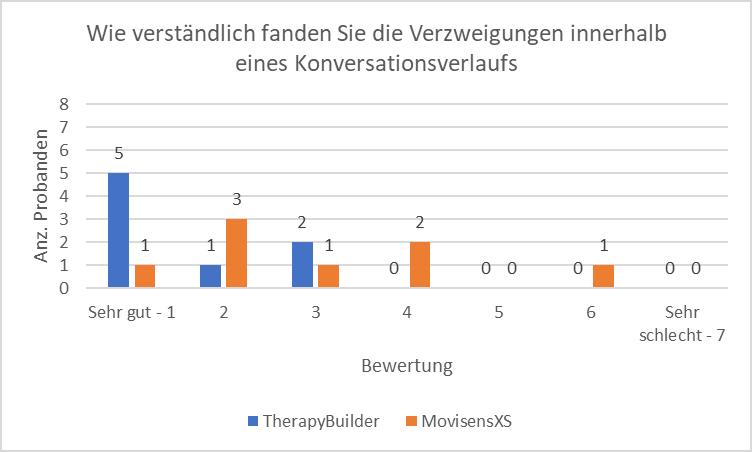
\includegraphics[width=1\textwidth]{pictures/diagramme/konvverzweig}
\caption{Architektur des \emph{konfiguration}}
\label{therapyBuilder}
\end{figure}

\begin{figure}[h]
\centering
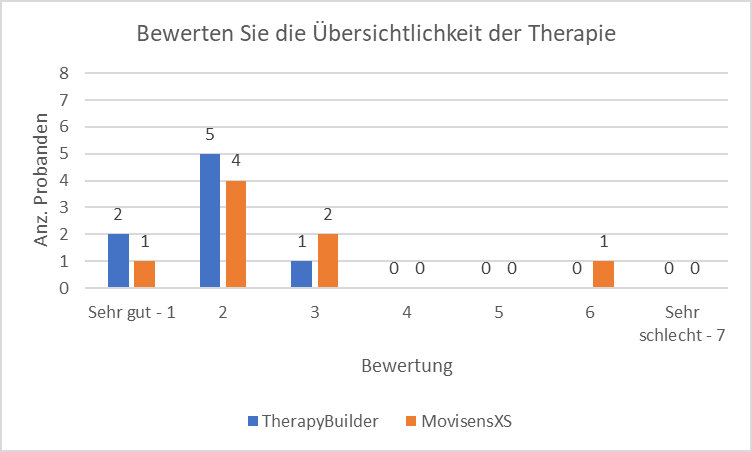
\includegraphics[width=1\textwidth]{pictures/diagramme/therapieuebersicht}
\caption{Architektur des \emph{konfiguration}}
\label{therapyBuilder}
\end{figure}

\begin{figure}[h]
\centering
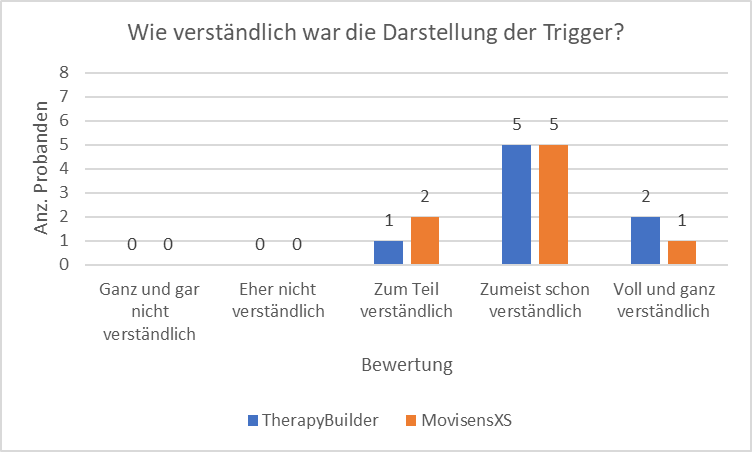
\includegraphics[width=1\textwidth]{pictures/diagramme/triggerdarstellung}
\caption{Architektur des \emph{konfiguration}}
\label{therapyBuilder}
\end{figure}

\begin{figure}[h]
\centering
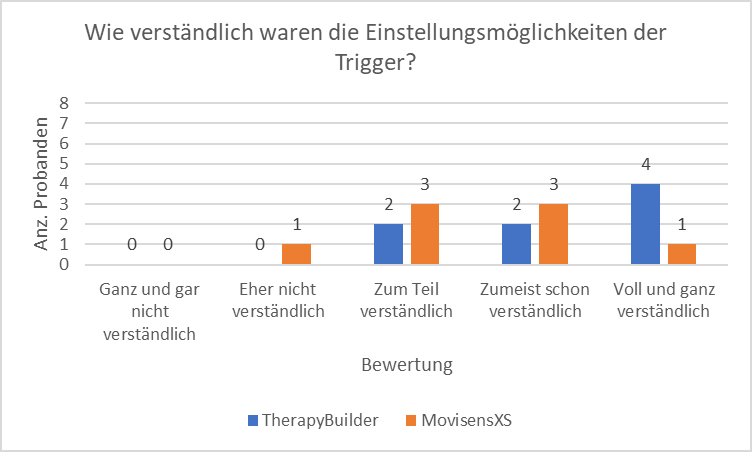
\includegraphics[width=1\textwidth]{pictures/diagramme/triggereinstellung}
\caption{Architektur des \emph{konfiguration}}
\label{therapyBuilder}
\end{figure}

\begin{figure}[h]
\centering
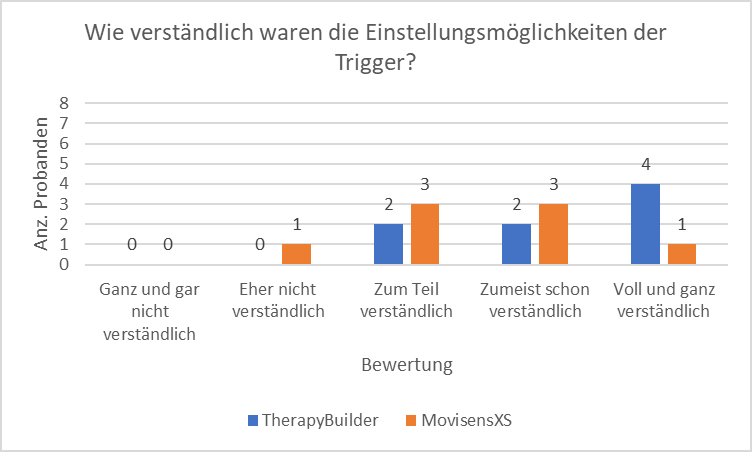
\includegraphics[width=1\textwidth]{pictures/diagramme/triggereinstellung}
\caption{Architektur des \emph{konfiguration}}
\label{therapyBuilder}
\end{figure}

\begin{figure}[h]
\centering
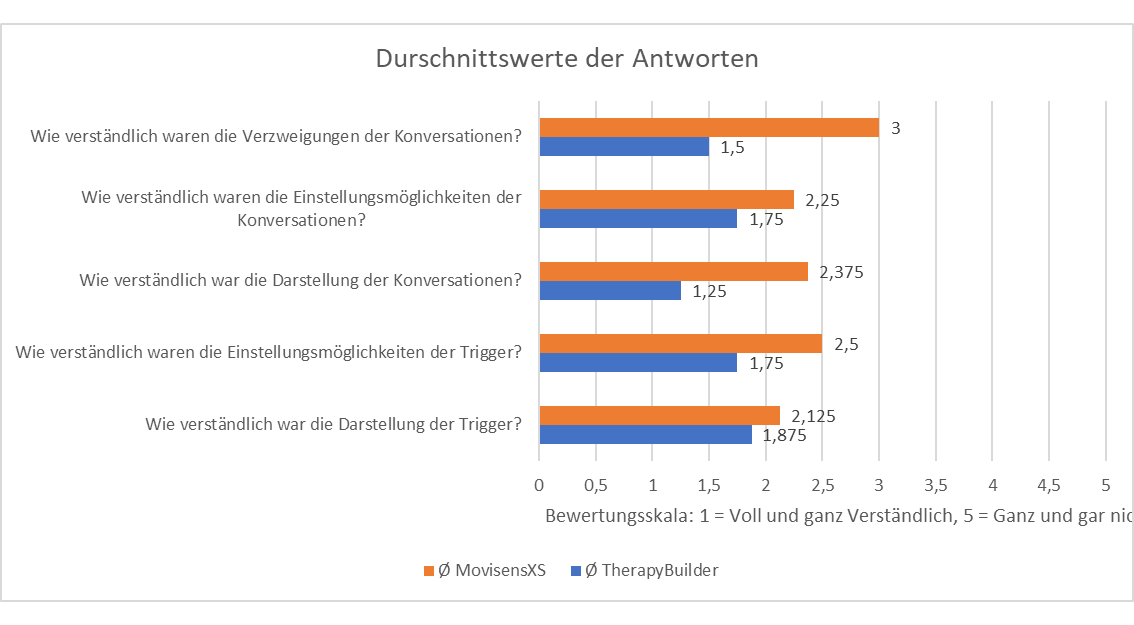
\includegraphics[width=1\textwidth]{pictures/diagramme/antwortendurchsch1}
\caption{Architektur des \emph{konfiguration}}
\label{therapyBuilder}
\end{figure}

\begin{figure}[h]
\centering
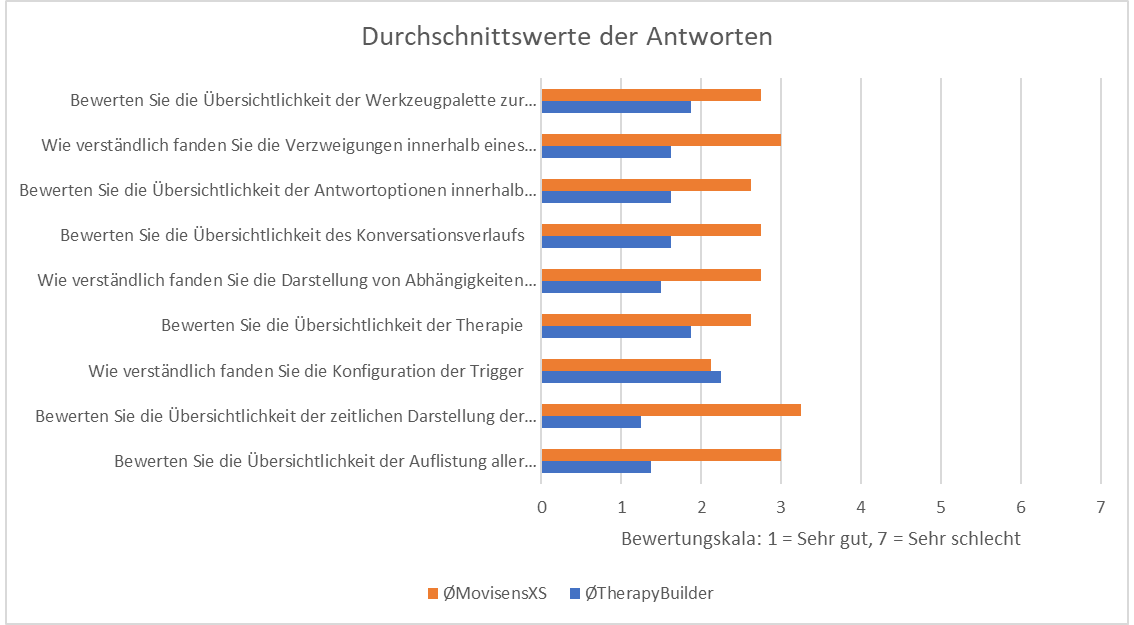
\includegraphics[width=1\textwidth]{pictures/diagramme/antwortendurchsch2}
\caption{Architektur des \emph{konfiguration}}
\label{therapyBuilder}
\end{figure}